\subsection{Linearization}

Before proceeding with the numerical solution of the system, we can try to linearize the system of equations to obtain a linear system of equations.
To do so, we can use a Taylor series expansion of the force-displacement relationship \ref{eq:force_displacement_relationship} around the point $\vec{u} = \vec{0}$.
A general Taylor series expansion of a function $f(x, y)$ around the point $(x_0, y_0)$ is given by:

\begin{align}
    f(x, y) & = f(x_0, y_0) + \nonumber                                                                                                                                                                                                                                  \\
            & + \frac{\partial f}{\partial x}(x_0, y_0) \cdot (x - x_0) + \frac{\partial f}{\partial y}(x_0, y_0) \cdot (y - y_0) + \nonumber                                                                                                                            \\
            & + \frac{1}{2} \frac{\partial^2 f}{\partial x^2}(x_0, y_0) \cdot (x - x_0)^2 + \frac{1}{2} \frac{\partial^2 f}{\partial y^2}(x_0, y_0) \cdot (y - y_0)^2 + \frac{\partial^2 f}{\partial x \partial y}(x_0, y_0) \cdot (x - x_0) \cdot (y - y_0) + \nonumber \\
            & + \dots
\end{align}

We can now try to apply the (1° order) Taylor series expansion to the force-displacement relationship \ref{eq:force_displacement_relationship} to obtain the following system of linear equations:

We can now try to apply the Taylor series expansion to the force-displacement relationship \ref{eq:force_displacement_relationship}.


\subsubsection{Taylor series of order 1}

By applying the Taylor series expansion of order 1, we obtain the following system of linear equations:

\begin{equation}
    \begin{Bmatrix}
        \widehat{\vec{P_x}} \\
        \widehat{\vec{P_y}}
    \end{Bmatrix}
    =
    \begin{Bmatrix}
        \frac{\text{A}_1 \text{E}_1 u}{\text{L}_1} \\
        \frac{\text{A}_2 \text{E}_2 v}{\text{L}_2}
    \end{Bmatrix}
\end{equation}


\subsubsection{Taylor series of order 2}

By applying the Taylor series expansion of order 2, we obtain the following system of quadratic equations:

\begin{equation}
    \begin{Bmatrix}
        \widehat{\widehat{\vec{P_x}}} \\
        \widehat{\widehat{\vec{P_y}}}
    \end{Bmatrix}
    =
    \begin{Bmatrix}
        \frac{\text{A}_1 \text{E}_1 u}{\text{L}_1}+\frac{\text{A}_2 \text{E}_2 v^2}{\text{L}_2^2}+\frac{\text{A}_1 \text{E}_1 \left(u^2+v^2\right)}{2 \text{L}_1^2} \\
        \frac{\text{A}_2 \text{E}_2 v}{\text{L}_2}+\frac{\text{A}_1 \text{E}_1 uv}{\text{L}_1^2}+\frac{\text{A}_2 \text{E}_2 \left(u^2+2 u v-v^2\right)}{2 \text{L}_2^2}
    \end{Bmatrix}
\end{equation}


\subsubsection{Taylor series of order 3}

By applying the Taylor series expansion of order 3, we obtain the following system of cubic equations:

\begin{equation}
    \begin{Bmatrix}
        \widehat{\widehat{\widehat{\vec{P_x}}}} \\
        \widehat{\widehat{\widehat{\vec{P_y}}}}
    \end{Bmatrix}
    =
    \begin{Bmatrix}
        \frac{\text{A}_1 \text{E}_1 u}{\text{L}_1}+\frac{\text{A}_2 \text{E}_2 v^2}{\text{L}_2^2}-\frac{\text{A}_1 \text{E}_1 u v^2}{2 \text{L}_1^3}-\frac{\text{A}_2 \text{E}_2 v \left(-u^2+v^2\right)}{2 \text{L}_2^3}+\frac{\text{A}_1 \text{E}_1 \left(u^2+v^2\right)}{2 \text{L}_1^2} \\
        \frac{\text{A}_2 \text{E}_2 v}{\text{L}_2}+\frac{\text{A}_1 \text{E}_1 u v}{\text{L}_1^2}+\frac{\text{A}_2 \text{E}_2 \left(u^2+2 u v-v^2\right)}{2 \text{L}_2^2}+\frac{\text{A}_1 \text{E}_1 v \left(-u^2+v^2\right)}{2 \text{L}_1^3}+\frac{\text{A}_2 \text{E}_2 \left(u^3-2 u^2 v-u v^2+v^3\right)}{2 \text{L}_2^3}
    \end{Bmatrix}
\end{equation}


\subsubsection{Comparison}

As it's easy to understand, the system of equations obtained with the Taylor series expansion of order 2 (since it has a higher order) is more accurate than the system of equations obtained with the Taylor series expansion of order 1.
We can now compare the results obtained with the two systems of equations to understand the error introduced by the linearization.
In the following figures, we can see the error introduced by the linearization with respect to the original force-displacement relationship \ref{eq:force_displacement_relationship}.

\begin{figure}[H]
    \centering
    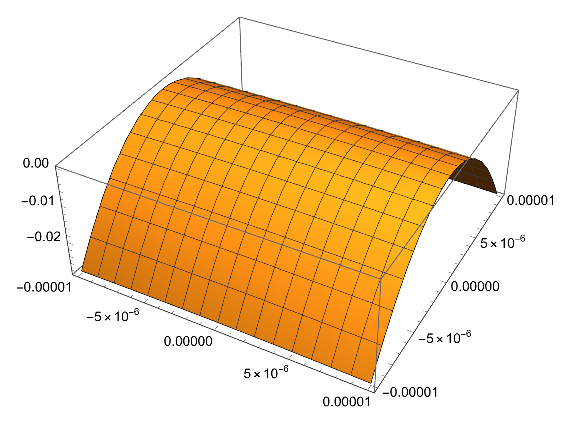
\includegraphics[width=.5\textwidth]{./pdf/residual_taylor_order_1}
    \caption{Error analysis for a Taylor series of order 1}
    \label{fig:residual_taylor_order_1}
\end{figure}

\begin{figure}[H]
    \centering
    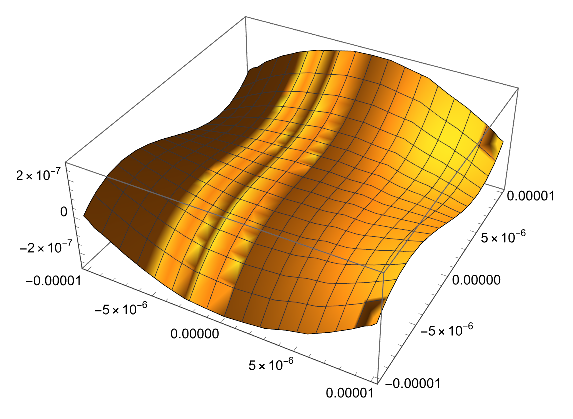
\includegraphics[width=.5\textwidth]{./pdf/residual_taylor_order_2}
    \caption{Error analysis for a Taylor series of order 2}
    \label{fig:residual_taylor_order_2}
\end{figure}

\begin{figure}[H]
    \centering
    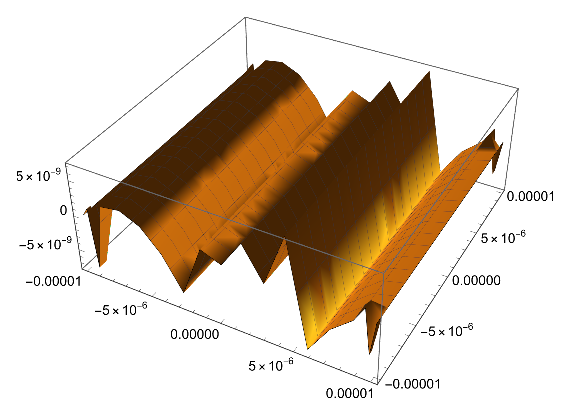
\includegraphics[width=.5\textwidth]{./pdf/residual_taylor_order_3}
    \caption{Error analysis for a Taylor series of order 3}
    \label{fig:residual_taylor_order_3}
\end{figure}

As we can see, around the point $\vec{u} = \vec{0}$, the error is negligible for both the approximations.
However, as we move away from the point $\vec{u} = \vec{0}$, the error introduced by the linearization increases.

In particular, we can see that the error introduced by the linearization decreases as we increase the order of the Taylor series expansion.